\subsection{ソフトウェアテストの基礎}
\subsubsection{欠陥と障害}
欠陥は、望ましくない振る舞いの原因である。障害は、その原因が実行時に表に出て、利用者や外部システムから観測される現象である。欠陥があっても、該当する入力や状態に到達しなければ障害として現れないことがある。逆に、障害が観測されても、どの欠陥が原因かを一意に決められるとは限らない。

\term{テスト}{Testing}が直接明らかにするのは、多くの場合、障害である。テストに失敗した後は、デバッグや原因分析によって欠陥を見つけ、修正する必要がある。したがって、「テスト」と「デバッグ」は連続して使われることが多いが、同じ活動ではない。テストは失敗を検出する活動であり、デバッグは原因を突き止めて直す活動である。

\begin{pointbox}{重要}
テストは、欠陥の存在を示すことはできるが、欠陥が存在しないことを一般には証明できない。現実のソフトウェアでは、完全な網羅テストが不可能だからである。
\end{pointbox}

\par\smallskip
\begin{center}
\centering
\IfFileExists{assets/generated_figures/ch05/fig-ch05-03.png}{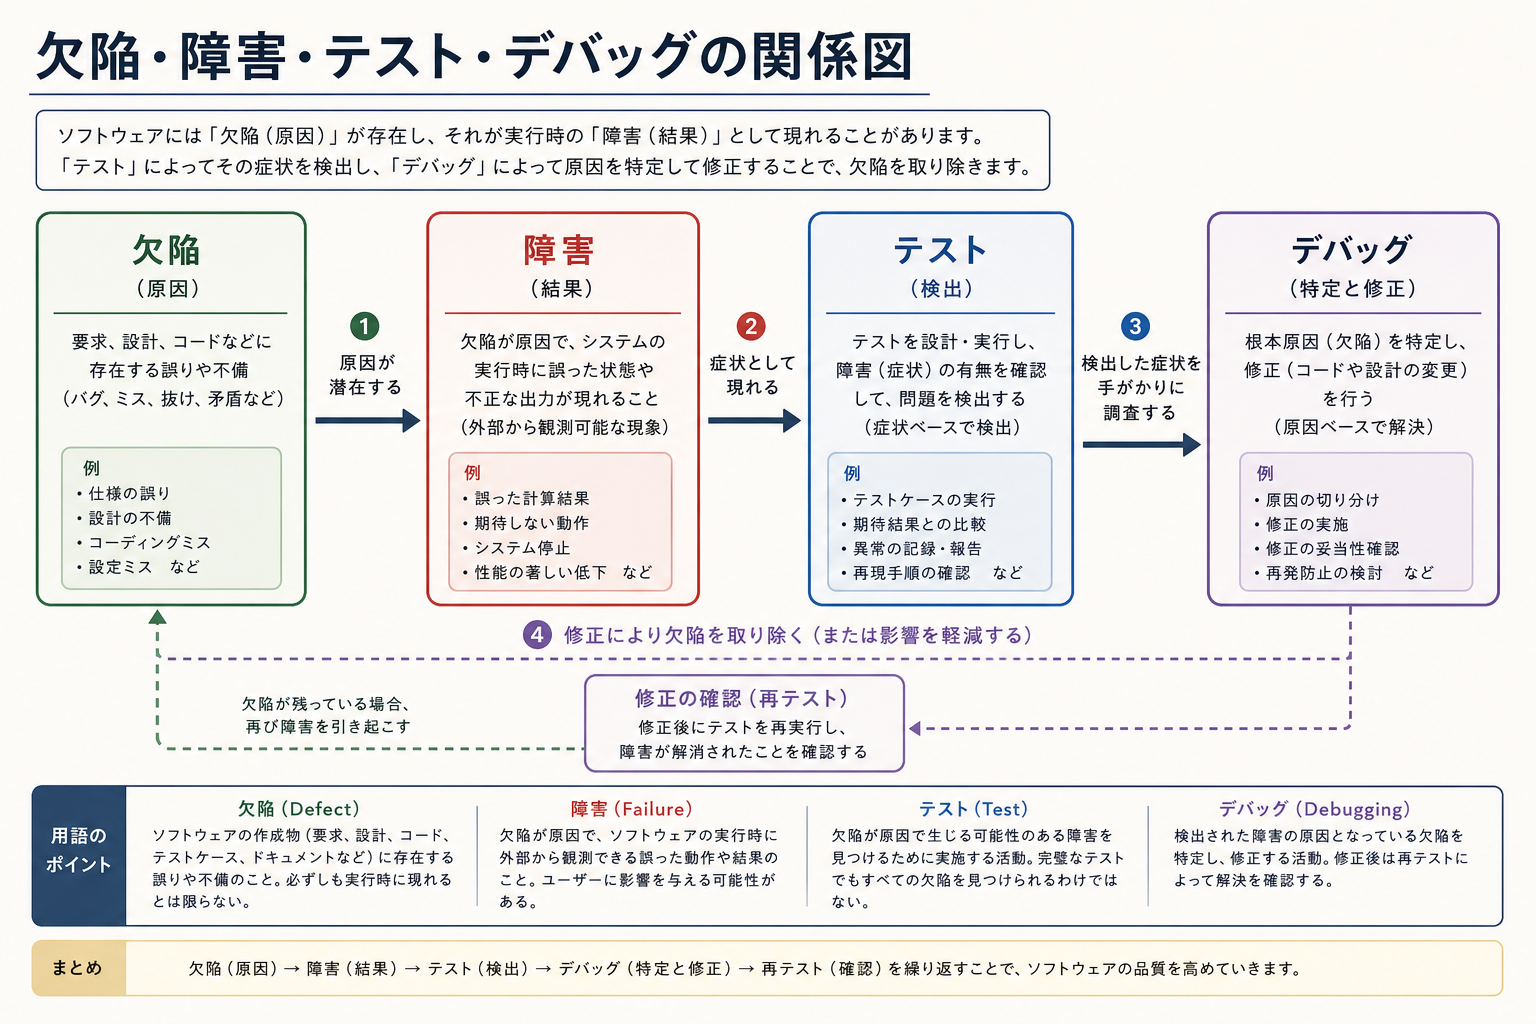
\includegraphics[width=0.96\linewidth]{assets/generated_figures/ch05/fig-ch05-03.png}}{\fbox{\parbox[c][48mm][c]{0.9\linewidth}{\centering 画像生成待ち\\欠陥・障害・テスト・デバッグの関係図}}}
\par\smallskip
\refstepcounter{figure}\label{fig:ch05-03}図 \thefigure: 欠陥・障害・テスト・デバッグの関係図
\end{center}
図 \thefigure は、欠陥・障害・テスト・デバッグの関係図を視覚的に整理したものである。
\par\smallskip

\subsubsection{主要論点}
\paragraph{テストケース作成}
テストケース作成とは、特定の目的に役立つテストスイートを作る活動である。目的は、十分性の確認、正確性の確認、法令や標準への適合評価などである。テストケース作成は手間が大きいため、自動生成、モデルベース生成、仕様からの導出、コード構造からの導出などの技法やツールが用いられる。

\paragraph{テスト選択と十分性基準}
テスト選択基準は、どのテストケースを選ぶかを決めるための基準である。テスト十分性基準は、どの程度まで実施すれば十分とみなすかを決める基準である。たとえば、全分岐を少なくとも一度通す、すべての機能要求を少なくとも一度検証する、主要なリスクをすべて扱う、などが考えられる。

\paragraph{優先順位付けと最小化}
テストケース優先順位付けは、実行順序を決める活動である。重要度、リスク、過去の欠陥検出率、コードカバレッジ、類似度などを使い、価値の高いテストから先に実行する。テストケース最小化は、冗長なテストケースを削り、テストスイートを小さくする活動である。目的は、効果をできるだけ保ちながら費用と時間を下げることである。

\paragraph{テスト目的}
テストは、目的によって選ぶ技法も評価方法も変わる。機能が仕様どおりかを確認するテスト、性能を測るテスト、セキュリティ上の弱点を探すテスト、利用者が使いやすいかを確認するテストでは、必要なテストケースも期待結果も異なる。目的を曖昧にしたままテストすると、「たくさん実行したが何を確認したかわからない」という状態になりやすい。

\paragraph{評価と認証}
評価や認証のためのテストでは、要求、法令、標準、契約に対する根拠を示す必要がある。テストケースがどの基準から導かれたか、どの構成のシステムで実行されたか、同じ手順で再現できるかが重要である。認証が必要な領域では、テスト結果だけでなく、プロセスや文書の管理も重視される。

\paragraph{品質保証と品質改善のためのテスト}
テストは、品質保証と品質改善にも使われる。品質保証では、要求された品質水準を満たしていることを示す根拠を作る。品質改善では、失敗、欠陥、傾向、弱点を把握し、次の設計、実装、プロセス改善につなげる。

\paragraph{オラクル問題}
オラクル問題とは、実行結果が正しいかどうかを判断することが難しい問題である。期待結果が明確な四則演算なら判断は容易である。しかし、推薦システム、画像認識、複雑な最適化、機械学習モデル、長時間運用システムでは、何を正しい結果とみなすかが難しい。オラクルを自動化することも、しばしば高コストである。

\paragraph{理論的・実践的制約}
テストには限界がある。代表的な限界は、完全な網羅ができないこと、成功したテストが欠陥の不存在を証明しないこと、運用環境を完全には再現できないこと、期待結果を決めるのが難しいこと、テストケースを増やすほど費用が増えることである。

\paragraph{実行不能経路の問題}
実行不能経路とは、制御フロー上は存在するように見えるが、どの入力でも実際には通れない経路である。構造ベーステストでは、経路を通すテストを作ろうとしても、実行不能経路があると達成できない。実行不能経路の特定は、テスト時間の削減やセキュリティ上の弱点分析にも関係する。

\paragraph{テスト容易性}
テスト容易性には二つの意味がある。第一に、対象がテストしやすい構造になっているかである。第二に、欠陥がある場合にテストスイートが障害を露出させやすいかである。観測しにくい内部状態、外部環境に強く依存する処理、再現性の低い並行処理は、テスト容易性を下げる。

\paragraph{テスト実行と自動化}
テスト自動化は、入力生成、実行、結果比較、ログ収集、レポート作成、回帰テストなどを支援する。自動化は有効であるが、すべてを自動化すればよいわけではない。期待結果が曖昧なテスト、探索的な確認、人間の評価が必要な使いやすさの確認では、人手の役割が残る。

\paragraph{拡張性}
拡張性は、負荷、取引数、データ量、利用者数、分散環境の複雑さが増えたときに、ソフトウェアが対応できる能力である。拡張性のテストでは、単に機能が動くかではなく、規模が増えたときの処理能力、安定性、資源使用量を確認する。

\paragraph{テスト有効性}
テスト有効性は、テストが目的にどれだけ役立ったかを表す。欠陥検出率、最初の障害を見つけるまでのテスト数、カバレッジ、信頼性向上、残存リスク低減などで評価される。目的が違えば、有効性の測り方も変わる。

\paragraph{制御可能性・再現性・一般化可能性}
制御可能性は、テスト条件をどの程度制御できるかである。再現性は、別の人が同じ手順で同じ結果を得られるかである。一般化可能性は、あるテスト結果が他の環境、利用者、設定にも当てはまるかである。研究でも実務でも、テスト結果を信頼するにはこの三つが重要である。

\paragraph{オフラインテストとオンラインテスト}
オフラインテストは、外部環境との直接的な相互作用を切り離してテストする。オンラインテストは、実際の利用環境や本番に近い環境と相互作用しながらテストする。オフラインは制御しやすく、オンラインは現実に近い。どちらも期待結果を用いて評価する。

\subsubsection{他の活動との関係}
ソフトウェアテストは、品質管理、形式的検証、デバッグ、プログラム構築、セキュリティ、見積り、法的責任と関係する。しかし、それらと同じではない。レビューや静的解析は実行しない確認であり、テストを補完する。形式的検証は数学的に性質を示す活動であり、テストとは根拠の作り方が異なる。デバッグは、テストで観測された障害の原因を探して直す活動である。
